%!TEX TS-program = xelatex
\documentclass[10pt,xcolor=dvipsnames,compress]{beamer}
\logo{
\includegraphics[height=1cm]{Duke_shield.png}}
\usepackage{beamerthemesplit}
\usecolortheme[cmyk={1.0,.69,0.0,.115}]{structure}
\usetheme[height=11mm]{Rochester}
\setbeamertemplate{items}[ball] 
\setbeamerfont{tablefont}{size=\tiny}
\setbeamerfont{quotefont}{size=\small}


\usepackage[export]{adjustbox}
\usepackage{etoolbox}
\usepackage{dcolumn}
\usepackage[scale=2]{ccicons}
\usepackage{color}

% math typesetting
\usepackage{array}
\usepackage{amsmath}
\usepackage{amssymb}
\usepackage{amsthm}
\usepackage{amsfonts}
\usepackage{relsize}
\usepackage{mathtools}
\usepackage{bm}

% tables
\usepackage{tabularx}
\usepackage{booktabs}
\usepackage{multicol}
\usepackage{multirow}

% graphics stuff
\usepackage{subfig}
\usepackage{graphicx}
\usepackage[space]{grffile} 
\usepackage{tikz}

% to change enumeration symbols begin{enumerate}[(a)]
%\usepackage{enumerate}

% square bracket matrices
\let\bbordermatrix\bordermatrix
\patchcmd{\bbordermatrix}{8.75}{4.75}{}{}
\patchcmd{\bbordermatrix}{\left(}{\left[}{}{}
\patchcmd{\bbordermatrix}{\right)}{\right]}{}{}

% easy command for boldface math symbols
\newcommand{\mbs}[1]{\boldsymbol{#1}}

% command for R package font
\newcommand{\pkg}[1]{{\fontseries{b}\selectfont #1}}

% approx iid
\newcommand\simiid{\stackrel{\mathclap{\normalfont\mbox{\tiny{iid}}}}{\sim}}

% references to graphics
\makeatletter
\def\input@path{{/Users/janus829/Dropbox/Research/netModels/summResults/}, {/Users/s7m/Dropbox/Research/netModels/summResults/}, {/Users/mdw/Dropbox/Research/Ongoing/netModels/summResults/}}
\graphicspath{{/Users/janus829/Dropbox/Research/netModels/summResults/}, {/Users/s7m/Dropbox/Research/netModels/summResults/},{/Users/mdw/Dropbox/Research/Ongoing/netModels/summResults/}}

\title[AMEN]{Embracing Network Interdependence in International Relations\thanks{Based upon joint works with Shahryar Minhas (Michigan State University), Peter Hoff (Duke University), Cassy L. Dorff (University of New Mexico), Max Gallop (University of Strathclyde), Juan Tellez (Duke University), Howard Liu (Duke University), \& Margaret Foster (Duke University).}
}
\author 
{Michael D. Ward\\ 
Department of Political Science, Duke University} 
%\vspace[*]{5 cm}
\date{Prepared presentation at the Department of Political Science, Texas A\&M University, November 5, 2017. }



\begin{document}
\frame{\titlepage}


\begin{frame}
\frametitle{Abstract}
\framesubtitle{An Abstract for a Talk?}
\begin{itemize}
\item Much international relations scholarship concerns dyads. Dyadic observations do not typically satisfy the conditional independence criterion required for many statistical approaches. As a result, studies often produce results with biased coefficient estimates and poorly calibrated standard errors. These biases have profound consequences for evaluating parametric models. 

\item We present an alternative, regression-based, approach that accounts for the dependencies complicating this type of analysis, and present a simulation exercise highlighting the model's ability to account for the dyadic dependencies. We replicate five prominent studies, comparing the standard approach to our alternative. 

\item Conventional methods overstate the effect of key variables, underestimate the uncertainties, and often lead researchers to faulty conclusions about the substantive importance of their variables. 

\item Our approach dominates in terms of out-of-sample cross-validations, rendering it more useful in forecasting applications and in modeling the data generating process behind outcomes of interest.
\end{itemize}
\end{frame}

\frame{\frametitle{Overview of Seminar}
\framesubtitle{Please, ask questions when you have them.}\tableofcontents}
%%%%%%%%%%%%%%%%%%%%%%%%%%%%%%%%%%%%%%%%%%%%%%%%%%%%%%%%%%%%
\section{The Setup}
\frame{
  \frametitle{Motivation}

  Relational data consists of 
  \begin{itemize}
    \item a set of units or nodes
    \item a set of measurements, $y_{ij}$, specific to pairs of nodes $(i,j)$ 
  \end{itemize}

  \centering
  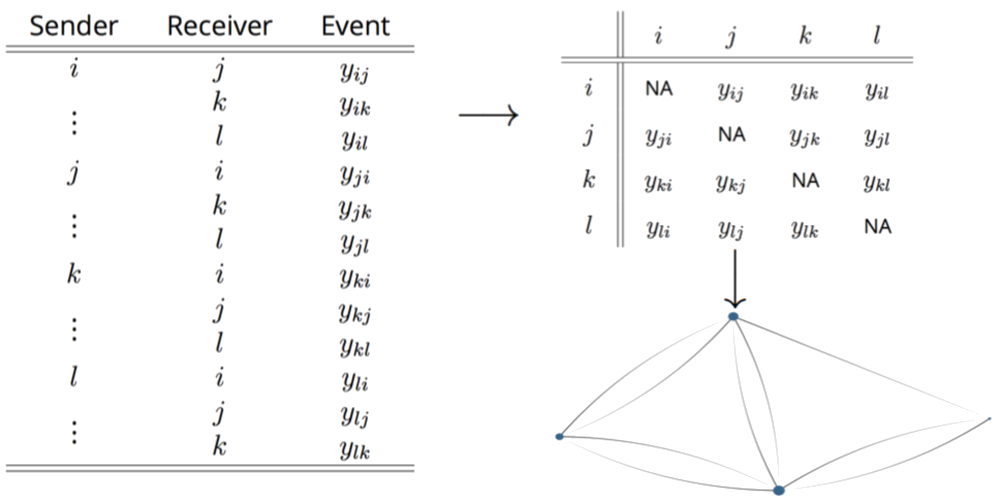
\includegraphics[width=1.05\textwidth]{df_adj_net3}
}
%%%%%%%%%%%%%%%%%%%%%%%%%%%%%%%%%%%%%%%%%%%%%%%%%%%%%%%%%%%%

%%%%%%%%%%%%%%%%%%%%%%%%%%%%%%%%%%%%%%%%%%%%%%%%%%%%%%%%%%%%
\frame{
  \frametitle{Relational data assumptions}

GLM: $y_{ij} \sim \beta^{T} X_{ij} + e_{ij}$

Networks typically show evidence against independence of {$e_{ij} : i \neq j$}

Not accounting for dependence can lead to:

\begin{itemize}
\item  biased effects estimation
\item  uncalibrated confidence intervals
\item  poor predictive performance
\item  inaccurate description of network phenomena
\end{itemize}

We've been hearing this concern for decades now:

\begin{tabular}{lll}
Thompson \& Walker (1982) & Beck et al. (1998) & Snijders (2011) \\
Frank \& Strauss (1986) & Signorino (1999) & Erikson et al. (2014) \\
Kenny (1996) & Li \& Loken (2002) & Aronow et al. (2015) \\
Krackhardt (1998) & Hoff \& Ward (2004) & Athey et al. (2016) \\
\end{tabular}

}
%%%%%%%%%%%%%%%%%%%%%%%%%%%%%%%%%%%%%%%%%%%%%%%%%%%%%%%%%%%%


%%%%%%%%%%%%%%%%%%%%%%%%%%%%%%%%%%%%%%%%%%%%%%%%%%%%%%%%%%%%
\frame{
  \frametitle{What network phenomena? Sender heterogeneity}

  Values across a row, say $\{y_{ij},y_{ik},y_{il}\}$, may be more similar to each other than other values in the adjacency matrix because each of these values has a common sender $i$

  \centering
  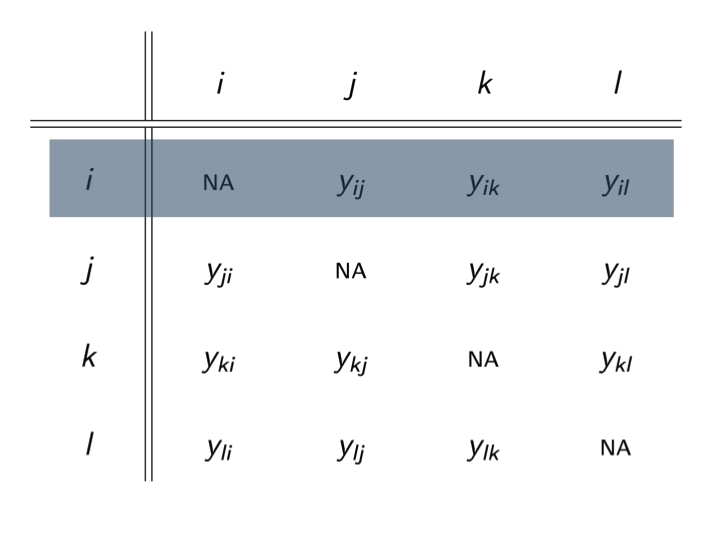
\includegraphics[width=.7\textwidth]{adjRowDep}

}
%%%%%%%%%%%%%%%%%%%%%%%%%%%%%%%%%%%%%%%%%%%%%%%%%%%%%%%%%%%%

%%%%%%%%%%%%%%%%%%%%%%%%%%%%%%%%%%%%%%%%%%%%%%%%%%%%%%%%%%%%
\frame{
  \frametitle{What network phenomena? Receiver heterogeneity}

  Values across a column, say $\{y_{ji},y_{ki},y_{li}\}$, may be more similar to each other than other values in the adjacency matrix because each of these values has a common receiver $i$

  \centering
  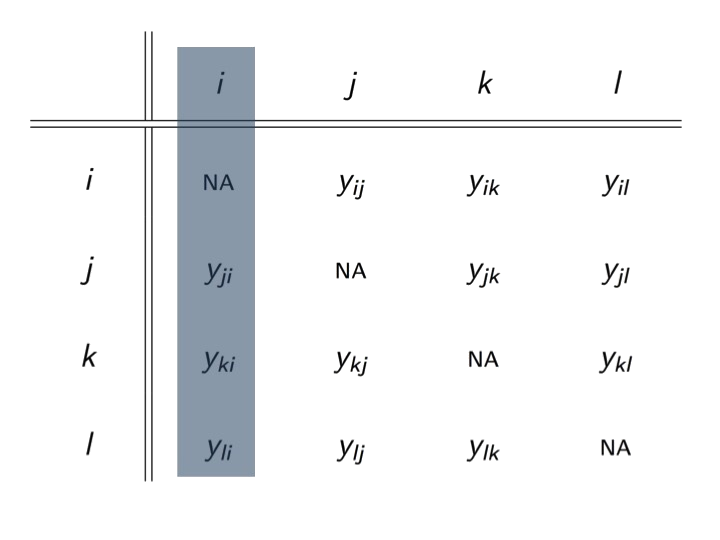
\includegraphics[width=.7\textwidth]{adjColDep}

}
%%%%%%%%%%%%%%%%%%%%%%%%%%%%%%%%%%%%%%%%%%%%%%%%%%%%%%%%%%%%

%%%%%%%%%%%%%%%%%%%%%%%%%%%%%%%%%%%%%%%%%%%%%%%%%%%%%%%%%%%%
\frame{
  \frametitle{What network phenomena? Sender-Receiver Covariance}

  Actors who are more likely to send ties in a network may also be more likely to receive them

  \centering
  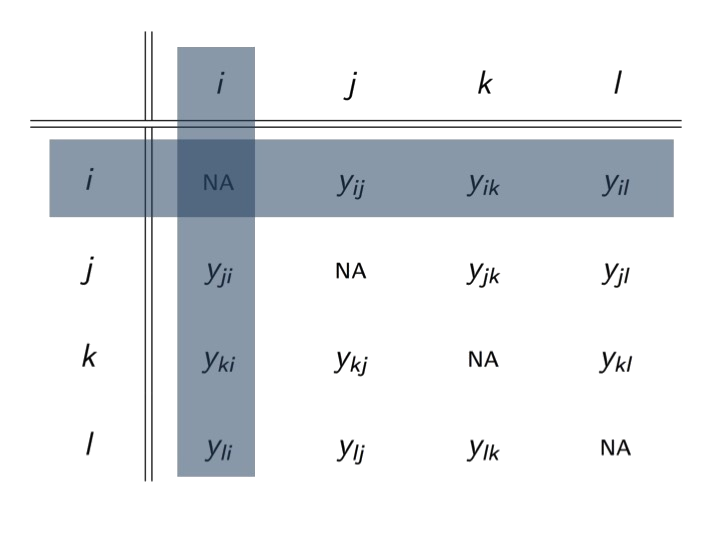
\includegraphics[width=.7\textwidth]{adjRowColCovar}

}
%%%%%%%%%%%%%%%%%%%%%%%%%%%%%%%%%%%%%%%%%%%%%%%%%%%%%%%%%%%%

%%%%%%%%%%%%%%%%%%%%%%%%%%%%%%%%%%%%%%%%%%%%%%%%%%%%%%%%%%%%
\frame{
  \frametitle{What network phenomena? Reciprocity}

  Values of $y_{ij}$ and $y_{ji}$ may be statistically dependent

  \centering
  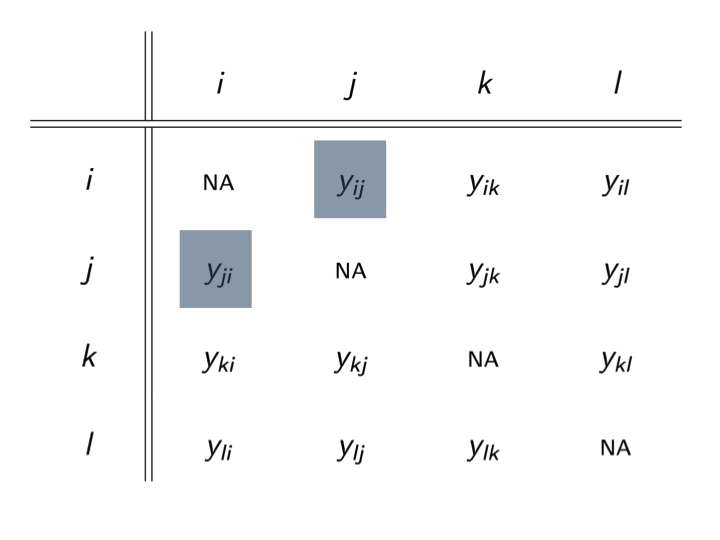
\includegraphics[width=.7\textwidth]{adjRecip}

}
%%%%%%%%%%%%%%%%%%%%%%%%%%%%%%%%%%%%%%%%%%%%%%%%%%%%%%%%%%%%
\section{The Social Relations Model}
%%%%%%%%%%%%%%%%%%%%%%%%%%%%%%%%%%%%%%%%%%%%%%%%%%%%%%%%%%%%
\frame{
  \frametitle{Social Relations Model (The ``A'' in AME)}

We use this model to form the additive effects portion of AME

\begin{align*}
\begin{aligned}
      y_{ij} &= \color{red}{\mu} + \color{red}{e_{ij}} \\
      e_{ij} &= a_{i} + b_{j} + \epsilon_{ij} \\
      \{ (a_{1}, b_{1}), \ldots, (a_{n}, b_{n}) \} &\sim N(0,\Sigma_{ab}) \\ 
      \{ (\epsilon_{ij}, \epsilon_{ji}) : \; i \neq j\} &\sim N(0,\Sigma_{\epsilon}), \text{ where } \\
      \Sigma_{ab} = \begin{pmatrix} \sigma_{a}^{2} & \sigma_{ab} \\ \sigma_{ab} & \sigma_{b}^2   \end{pmatrix} \;\;\;\;\; &\Sigma_{\epsilon} = \sigma_{\epsilon}^{2} \begin{pmatrix} 1 & \rho \\ \rho & 1  \end{pmatrix}
\end{aligned}
\end{align*}

\begin{itemize}
\item $\mu$ baseline measure of network activity
\item $e_{ij}$ residual variation that we will use the SRM to decompose
\end{itemize}

}
%%%%%%%%%%%%%%%%%%%%%%%%%%%%%%%%%%%%%%%%%%%%%%%%%%%%%%%%%%%%

%%%%%%%%%%%%%%%%%%%%%%%%%%%%%%%%%%%%%%%%%%%%%%%%%%%%%%%%%%%%
\frame{
  \frametitle{Social Relations Model (The ``A'' in AME)}

\begin{align*}
\begin{aligned}
      y_{ij} &= \mu + e_{ij} \\
      e_{ij} &= {\color{red}{a_{i} + b_{j}}} + \epsilon_{ij} \\
      \color{red}{\{ (a_{1}, b_{1}), \ldots, (a_{n}, b_{n}) \}} &\sim N(0,\Sigma_{ab}) \\ 
      \{ (\epsilon_{ij}, \epsilon_{ji}) : \; i \neq j\} &\sim N(0,\Sigma_{\epsilon}), \text{ where } \\
      \Sigma_{ab} = \begin{pmatrix} \sigma_{a}^{2} & \sigma_{ab} \\ \sigma_{ab} & \sigma_{b}^2   \end{pmatrix} \;\;\;\;\; &\Sigma_{\epsilon} = \sigma_{\epsilon}^{2} \begin{pmatrix} 1 & \rho \\ \rho & 1  \end{pmatrix}
\end{aligned}
\end{align*}

\begin{itemize}
\item  row/sender effect ($a_{i}$) \& column/receiver effect ($b_{j}$)
\item  Modeled jointly to account for correlation in how active an actor is in sending and receiving ties
\end{itemize}

}
%%%%%%%%%%%%%%%%%%%%%%%%%%%%%%%%%%%%%%%%%%%%%%%%%%%%%%%%%%%%

%%%%%%%%%%%%%%%%%%%%%%%%%%%%%%%%%%%%%%%%%%%%%%%%%%%%%%%%%%%%
\frame{
  \frametitle{Social Relations Model (The ``A'' in AME)}

\begin{align*}
\begin{aligned}
      y_{ij} &= \mu + e_{ij} \\
      e_{ij} &= a_{i} + b_{j} + \epsilon_{ij} \\
      \{ (a_{1}, b_{1}), \ldots, (a_{n}, b_{n}) \} &\sim N(0,\color{red}{\Sigma_{ab}}) \\ 
      \{ (\epsilon_{ij}, \epsilon_{ji}) : \; i \neq j\} &\sim N(0,\Sigma_{\epsilon}), \text{ where } \\
      \color{red}{\Sigma_{ab}} = \begin{pmatrix} \sigma_{a}^{2} & \sigma_{ab} \\ \sigma_{ab} & \sigma_{b}^2   \end{pmatrix} \;\;\;\;\; &\Sigma_{\epsilon} = \sigma_{\epsilon}^{2} \begin{pmatrix} 1 & \rho \\ \rho & 1  \end{pmatrix}
\end{aligned}
\end{align*}

\begin{itemize}
\item $\sigma_{a}^{2}$ and $\sigma_{b}^{2}$ capture heterogeneity in the row and column means
\item $\sigma_{ab}$ describes the linear relationship between these two effects (i.e., whether actors who send [receive] a lot of ties also receive [send] a lot of ties)
\end{itemize}

}
%%%%%%%%%%%%%%%%%%%%%%%%%%%%%%%%%%%%%%%%%%%%%%%%%%%%%%%%%%%%

%%%%%%%%%%%%%%%%%%%%%%%%%%%%%%%%%%%%%%%%%%%%%%%%%%%%%%%%%%%%
\frame{
  \frametitle{Social Relations Model (The ``A'' in AME)}

\begin{align*}
\begin{aligned}
      y_{ij} &= \mu + e_{ij} \\
      e_{ij} &= a_{i} + b_{j} + \color{red}{\epsilon_{ij}} \\
      \{ (a_{1}, b_{1}), \ldots, (a_{n}, b_{n}) \} &\sim N(0,\Sigma_{ab}) \\ 
      \color{red}{\{ (\epsilon_{ij}, \epsilon_{ji}) : \; i \neq j\}} &\sim N(0,\color{red}{\Sigma_{\epsilon}}), \text{ where } \\
      \Sigma_{ab} = \begin{pmatrix} \sigma_{a}^{2} & \sigma_{ab} \\ \sigma_{ab} & \sigma_{b}^2   \end{pmatrix} \;\;\;\;\; & \color{red}{\Sigma_{\epsilon}} = \sigma_{\epsilon}^{2} \begin{pmatrix} 1 & \rho \\ \rho & 1  \end{pmatrix}
\end{aligned}
\end{align*}

\begin{itemize}
\item  $\epsilon_{ij}$ captures the within dyad effect
\item  Second-order dependencies are described by $\sigma_{\epsilon}^{2}$
\item  Reciprocity, aka within dyad correlation, represented by $\rho$
\end{itemize}
}
%%%%%%%%%%%%%%%%%%%%%%%%%%%%%%%%%%%%%%%%%%%%%%%%%%%%%%%%%%%%

%%%%%%%%%%%%%%%%%%%%%%%%%%%%%%%%%%%%%%%%%%%%%%%%%%%%%%%%%%%%
\frame{
  \frametitle{Third-Order Dependencies}

  \vspace{-10mm}

  \begin{table}[ht]
  \begin{tabular}{lcr}
  \scshape{Homophily} & & \scshape{Stochastic Equivalence} \\
  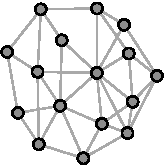
\includegraphics[width=.33\textwidth]{homophNet} & \hspace{2cm} &
  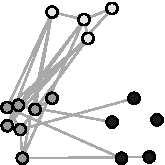
\includegraphics[width=.33\textwidth]{stochEquivNet}  
  \end{tabular}
  \end{table}

  To account for these patterns we can build on what we have so far and find an expression for $\gamma$:
  
  \vspace{-5mm}
  \begin{align*}
  \centering
  y_{ij} &\approx \beta^{T} X_{ij} + a_{i} + b_{j} + \gamma(u_{i},v_{j})
  \end{align*}

}
%%%%%%%%%%%%%%%%%%%%%%%%%%%%%%%%%%%%%%%%%%%%%%%%%%%%%%%%%%%%
\section{The Latent Factor Model}
%%%%%%%%%%%%%%%%%%%%%%%%%%%%%%%%%%%%%%%%%%%%%%%%%%%%%%%%%%%%


\frame{
  \frametitle{What Exactly Is Third-Order Dependency?}
  \framesubtitle{People Want to Know!}
\begin{itemize}
\item<1> If each node has individual characteristics, 
say $x_i$ and $x_j$ for two nodes.  Then,
$x_i \times x_j$ is the multiplicative product of their nodal characteristics and may be related to their relationship, 
$y_{ij}$.  
Let $x$ be an encoding of whether a node is democratic or not. 
Then, $x_i \times x_j \equiv 1 \iff$ 
\textit{both are democracies}.  This approach is often used in standard analyses as a variable often known as 
\textit{joint democracy}.  In the context of networks, a positive effect from the interaction of $x_i$ and $x_j$ might affect some dyadic variable, such as not being in a militarized dispute against one another---often denoted the democratic peace.  This positive effect is known in network terminology as \textit{homophily}.
Most studies just look at the correlation between aggregated variables, but the proposed approach can more directly estimate the degree of homophily.
\end{itemize}
}

\frame{
  \frametitle{What Exactly Is Third-Order Dependency?}
  \framesubtitle{People Want to Know!}
\begin{itemize}
\item<1> Homophily which stems from nodal characteristics results in certain types of network structures: 1) transitivity, 2) balance, and 3) clustering.  For example, homophily tends to induce a large number of \textit{triads}, since if $i$ is similar to $j$ and as a result has a link with $j$, for the same reason it will share a link with $k$ if $j$ and $k$ are similar, thus creating a triad.  Groups of triads tend to result in \textit{clusters}. This can result in clusters in which many elements in the cluster are not only related to one another but share similar characteristics.  This is known as \textit{stochastic equivalence}.

\item To capture this kind of stochastic equivalence---and other types of triadic dependence---we include a latent representation of nodal characteristics in the regression model.  This allows the network representation in a matrix to be dependent upon how similar these latent characteristics are. These latent nodal characteristics are represented by a type of multiplicative effects that are expressed as $\mathbf{u}_i^\intercal \mathbf{v}_i$.  This captures the third-order dependencies, i.e., the dependencies among triads.
\end{itemize}
}

\frame{
  \frametitle{Latent Factor Model: The ``M'' in AME}

Each node $i$ has an unknown latent factor

\vspace{-5mm}
\begin{align*}
{\textbf{u}_{i},\textbf{v}_{j}} \in \mathbb{R}^{k} \;\; i,j \in \{1, \ldots, n \} \\
\end{align*}

\vspace{-5mm}
The probability of a tie from $i$ to $j$ depends on their latent factors

\vspace{-5mm}
\begin{align*}
\begin{aligned}
  \gamma(\textbf{u}_{i}, \textbf{v}_{j}) &= \textbf{u}_{i}^{T} D \textbf{v}_{j} \\
  &= \sum_{k \in K} d_{k} u_{ik} v_{jk} \\
  &D \text{ is a  } K \times K \text{ diagonal matrix}
\end{aligned}
\end{align*}

This can account for both stochastic equivalence and homophily, as well as clustering and balance.

}


\frame{
  \frametitle{How Does Estimation Work?}
  \framesubtitle{It Is NOT All in the Error Term!}
 \begin{itemize}
  \item sample $\bm\theta \; | \;  \bm\beta, \mathbf{X}, \bm\theta, \mathbf{a}, \mathbf{b}, \mathbf{U}, \mathbf{V}, \Sigma_{ab}, \rho, \text{ and } \sigma_{\epsilon}^{2}$ (Normal)
  \item sample $\bm\beta \; | \;  \mathbf{X}, \bm\theta, \mathbf{a}, \mathbf{b}, \mathbf{U}, \mathbf{V}, \Sigma_{ab}, \rho, \text{ and } \sigma_{\epsilon}^{2}$ (Normal)
  \item sample $\mathbf{a}, \mathbf{b} \; | \; \bm\beta, \mathbf{X}, \bm\theta, \mathbf{U}, \mathbf{V}, \Sigma_{ab}, \rho, \text{ and } \sigma_{\epsilon}^{2}$ (Normal)
  \item sample $\Sigma_{ab} \; | \; \bm\beta, \mathbf{X}, \bm\theta, \mathbf{a}, \mathbf{b}, \mathbf{U}, \mathbf{V}, \rho, \text{ and } \sigma_{\epsilon}^{2}$ (Inverse-Wishart)
  \item update $\rho$ using a Metropolis-Hastings step with proposal $p^{*} | p  \sim$ truncated normal$_{[-1,1]}(\rho, \sigma_{\epsilon}^{2})$
  \item sample $\sigma_{\epsilon}^{2} \; | \; \bm\beta, \mathbf{X}, \bm\theta, \mathbf{a}, \mathbf{b}, \mathbf{U}, \mathbf{V}, \Sigma_{ab}, \text{ and } \rho$ (Inverse-Gamma)
  \item For each $k \in K$:
  \begin{itemize}
    \item Sample $\mathbf{U}_{[,k]} \; | \; \bm\beta, \mathbf{X}, \bm\theta, \mathbf{a}, \mathbf{b}, \mathbf{U}_{[,-k]}, \mathbf{V}, \Sigma_{ab}, \rho, \text{ and } \sigma_{\epsilon}^{2}$ (Normal)
    \item Sample $\mathbf{V}_{[,k]} \; | \; \bm\beta, \mathbf{X}, \bm\theta, \mathbf{a}, \mathbf{b}, \mathbf{U}, \mathbf{V}_{[,-k]}, \Sigma_{ab}, \rho, \text{ and } \sigma_{\epsilon}^{2}$ (Normal)
    \item Sample $\mathbf{D}_{[k,k]}  \; | \; \bm\beta, \mathbf{X}, \bm\theta,\mathbf{a}, \mathbf{b}, \mathbf{U}, \mathbf{V}, \Sigma_{ab}, \rho, \text{ and } \sigma_{\epsilon}^{2}$ (Normal)\footnote{Subsequent to estimation, $\mathbf{D}$ matrix is absorbed into the calculation for $\mathbf{V}$ as we iterate through $K$. }
  \end{itemize}
 \end{itemize}
  
}
%%%%%%%%%%%%%%%%%%%%%%%%%%%%%%%%%%%%%%%%%%%%%%%%%%%%%%%%%%%%
\section{Simulation of AME}
\frame{
  \frametitle{Simulation Comparing GLM and LFM}
  \framesubtitle{}
We utilize a simulation study to highlight the utility of AME as an inferential tool for dyadic analysis. The goal of the simulation is to assess how well AME can provide unbiased and well-calibrated estimates of coefficient parameters in the presence of unobserved dependencies. Specifically, we are concerned with conducting inference on regression parameters of a linear model for a network in the case where there is an omitted variable. For instance, assume that the true data-generating process for a particular $Y$ is given by:

\begin{align}
  y_{i,j} \sim  \mu + \beta x_{i,j} + \gamma w_{i,j} + \epsilon_{i,j}
  \label{eqn:sim}
\end{align}
where $Y= \{y_{i,j}\}\in \mathbb R^{n\times n}$ is an observed sociomatrix, $X = \{x_{i,j} \} \in \mathbb R^{n \times n}$ is a matrix of observed dyad-specific characteristics, and $W = \{ w_{i,j}\} \in \mathbb R^{n \times n}$ is a matrix of unobserved dyad-specific characteristics. $Y$ can be thought of as a dyadic dependent variable, $X$ and $W$ are both dyadic covariates that are a part of the data-generating process for $Y$, but $W$ is not observed.
}

\frame{
  \frametitle{Simulation Comparing GLM and LFM}
  \framesubtitle{Three Alternatives:}

\begin{itemize}
  \item the standard international relations approach assuming independent errors (current state-of-the discipline); 
  \item the AME approach with a unidimensional latent factor space ($K=1$);
  \item an ``oracle'' regression model that assumes we have measured all sources of dependencies and thus includes both $x_{i,j}$ and $w_{i,j}$. 
\end{itemize}

For the simulation we set the true value of $\mu$ (the intercept term) to -2 and $\beta$ (the effect of $X$ on $Y$) to 1. The value of $\gamma$ is also set to 1, which corresponds to an example where $W$ is associated with homophily. 
}


\frame{
  \frametitle{Regression Parameters from Simulations}
  \framesubtitle{}
\begin{figure}
  \centering
  \caption{Regression parameter estimates for the naive, AME, and oracle models from 1,000 simulations. Summary statistics are presented through a traditional box plot, and the estimates from each simulation are visualized as well as points.}
  \label{fig:ameBias}
  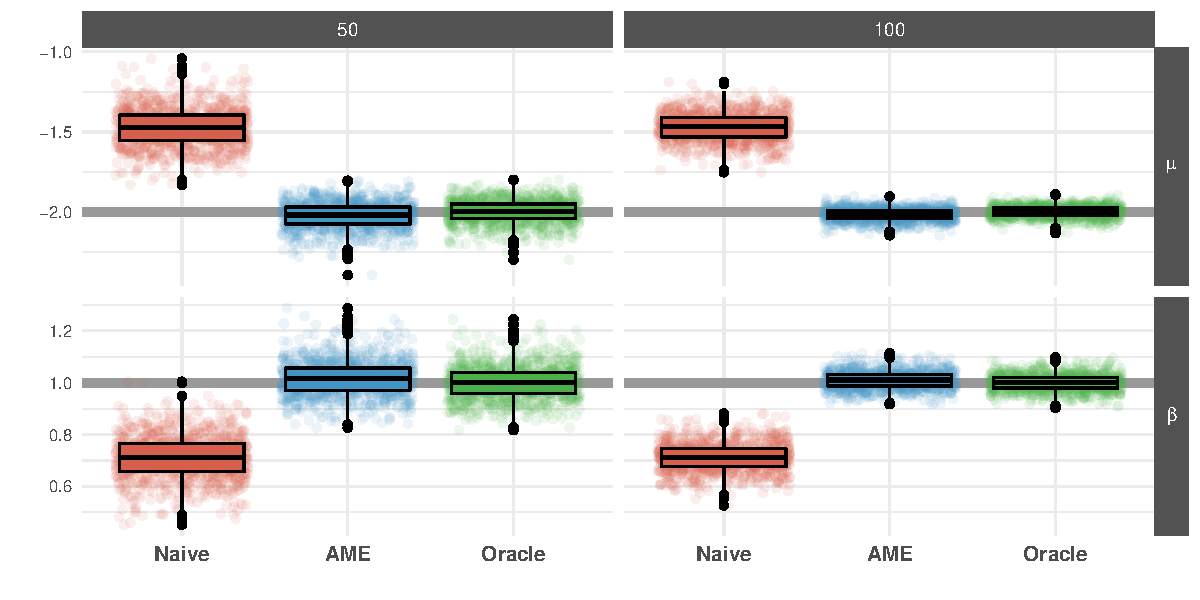
\includegraphics[width=\textwidth]{ameSimBias_all.pdf} \\
\end{figure}
}
%
\frame{
  \frametitle{Coverage in the Simulations}
  \framesubtitle{}
\begin{figure}
  \centering
  \caption{Proportion of times the true value fell within the estimated 95\% confidence interval for the naive, AME, and oracle models from 1,000 simulations.}
  \label{fig:ameCalib}
  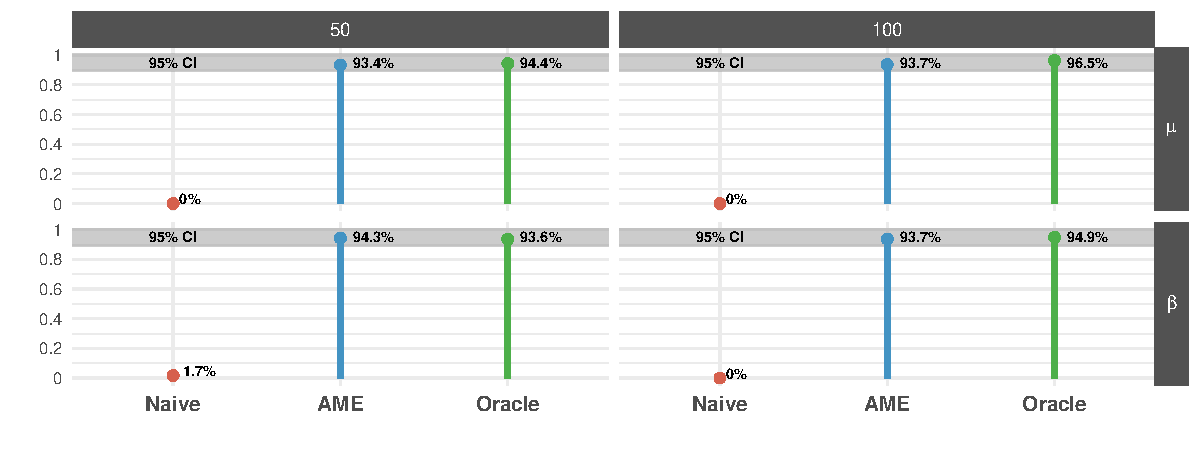
\includegraphics[width=\textwidth]{ameSimCover_all.pdf} \\
\end{figure}
}
%%%%%%%%%%%%%%%%%%%%%%%%%%%%%%%%%%%%%%%%%%%%%%%%%%%%%%%%%%%
\section{Five Easy Pieces: Replication with AME}
%%%%%%%%%%%%%%%%%%%%%%%%%%%%%%%%%%%%%%%%%%%%%%%%%%%%%%%%%%%%
\frame{
    \frametitle{Does it Really Matter?}
  \framesubtitle{Let's Look at Five Recent Publications in IR}

\begin{table}
\caption{Features of the Studies Re-estimated.}
\scalebox{.7}{
  \begin{tabular}{lcccccc}
    & Model &  Date Range & N. Actors  & N. Dyads & Dyads Type & Clustering $\sigma_{\hat{\beta}}$ \\ \toprule
    Reiter \& Stam (JCR; 2003) &Logit &1945--1995 &  193 & $753,456$ & Directed & Robust \\  
    McDonald (JCR; 2004) & Logit &1959--2002 & 198 & $92,354$ & Undirected & Robust\\
    Rose (AER; 2004) & OLS & 1948--1999 & 177 & $234,597$ & Directed & Robust \\  
    Weeks (APSR; 2012) & Logit & 1946--1999 &197 &  $901,540$ & Directed & Robust \\
    Gibler (APSR; 2017) & Logit & 1816--2008 &193 &   $650,557$ & Undirected & none \\ \bottomrule
  \end{tabular}
  }
\end{table} 
}

\frame{
    \frametitle{Does it Really Matter?}
  \framesubtitle{Some Deets}
\begin{table}[ht]
\centering
\caption{Here we provide a brief summary of the key variable in each of the five replications and a note about whether or not the finding is replicated when using our network-based approach.}
\scalebox{.7}{
  \begin{tabular}{l p{7cm} l} \toprule
    \multirow{2}{*}{Study} & \multirow{2}{*}{Central Finding} &  Replicates \\ 
      & &  in a Network Model? \\ \toprule
    Reiter \& Stam (2003) & Personalist Regimes Attack Democracies, Not Vice Versa & {Does Not Replicate} \\ \midrule
    McDonald (2004) & Lower Trade Barriers and Higher Trade Lead to Peace & {Does Not Replicate}\\ \midrule
    Rose (2004) & WTO Membership Does not Affect Trade & {Partially Replicates}\\ \midrule
    Weeks (2012) & Bosses, Juntas, and Strongmen are more Aggressive; Machines are Not & {Does Not Replicate} \\\midrule
    Gibler (2017) & Power Parity at Time of Entry to International System Inceases Conflict & {Does Not Replicate}\\ \bottomrule
  \end{tabular}
  }
  \label{tab:modelFindingSumm}
\end{table}
}

\frame{
  \frametitle{Performance Statistics}
  \framesubtitle{In out-of-sample tests}
\vspace{-5mm}
\begin{table}[ht]
\scalebox{.7}{
  \begin{tabular}{ll cc}  \toprule
  Study & Statistic & GLM & AME \\
  \midrule
\multirow{2}{*}{Reiter \& Stam (2003)} & Area Under ROC Curve, AUC-ROC & 0.92 & {0.96} \\
    ~ & Area Under PR Curve, AUC-PR & 0.08 &  {0.15} \\   \midrule
\multirow{2}{*}{McDonald (2004)} & AUC-ROC & 0.92 &  {0.99} \\
    ~ & AUC-PR & 0.13 &  {0.28} \\    \midrule
\multirow{2}{*}{Rose (2004)} & RMSE & 3.23 &  {1.99} \\
    ~ & RMDSE & 2.01 &  {1.06} \\ \midrule
\multirow{2}{*}{Weeks (2012)} & AUC-ROC & 0.64 &  {0.97} \\
    ~ & AUC-PR & 0.00 &  {0.15} \\    \midrule
\multirow{2}{*}{Gibler (2017)} & AUC-ROC & 0.52 &  {0.91} \\
    ~ & AUC-PR & 0.00 &  {0.08} \\      \bottomrule
  \end{tabular}
  }
\end{table}
}

\frame{
  \frametitle{Reiter-Stam Performance Comparisons}
  \framesubtitle{ }
\vspace{-5mm}
\begin{figure}
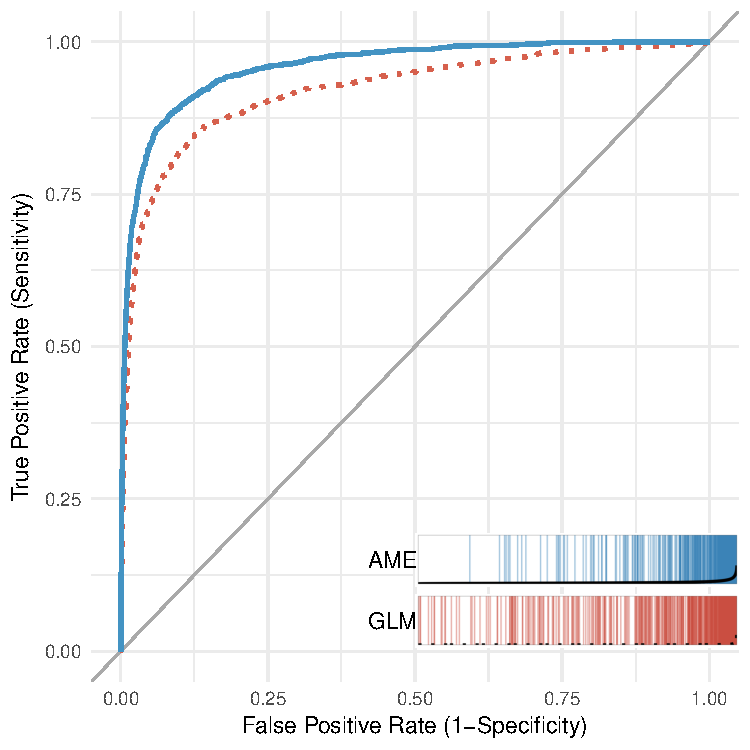
\includegraphics[height=5cm]{rsroc}
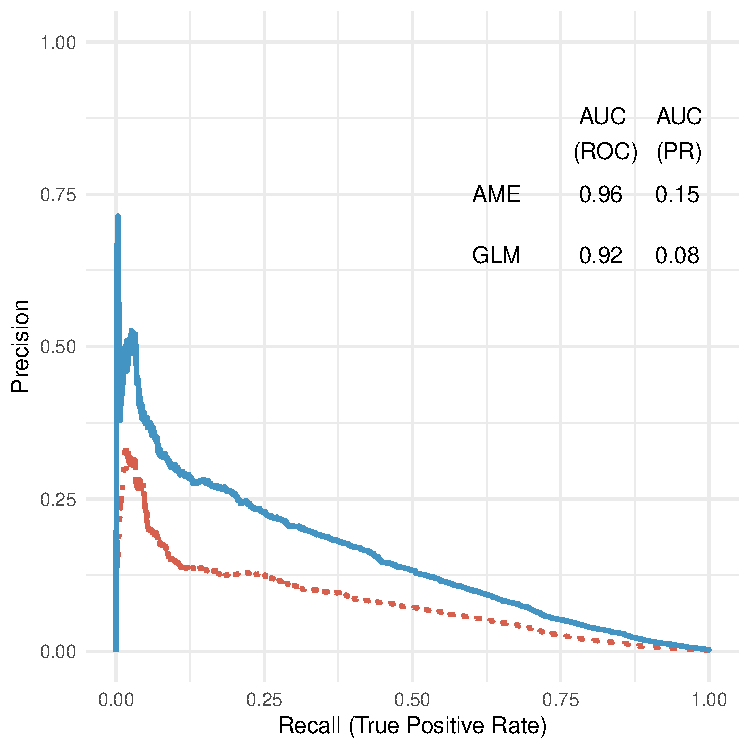
\includegraphics[height=5cm]{rspr}
\caption{Reiter-Stam Performance}
\end{figure}
}

\frame{
  \frametitle{McDonald Performance Comparisons }
  \framesubtitle{ }
\vspace{-5mm}
\begin{figure}
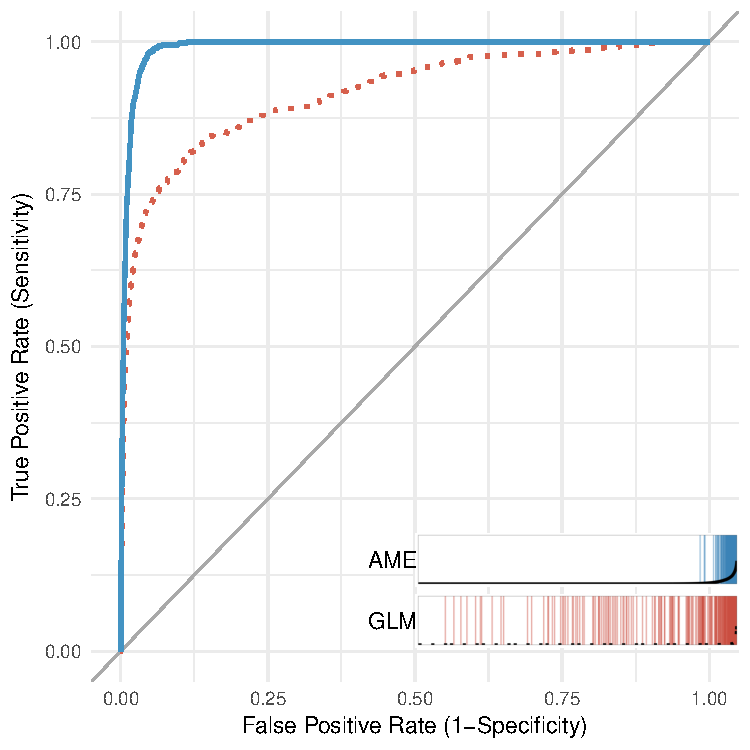
\includegraphics[height=5cm]{mcdonaldroc}
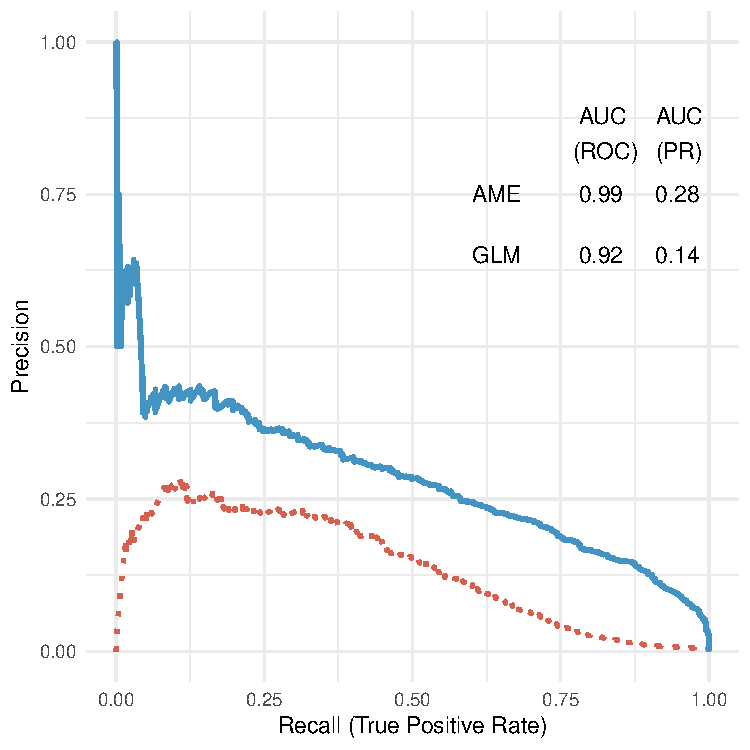
\includegraphics[height=5cm]{mcdonaldpr}
\caption{McDonald Performance }
\end{figure}
}

\frame{
  \frametitle{Rose Performance Comparisons }
  \framesubtitle{ }
%\vspace{-7.5mm}
\begin{figure}
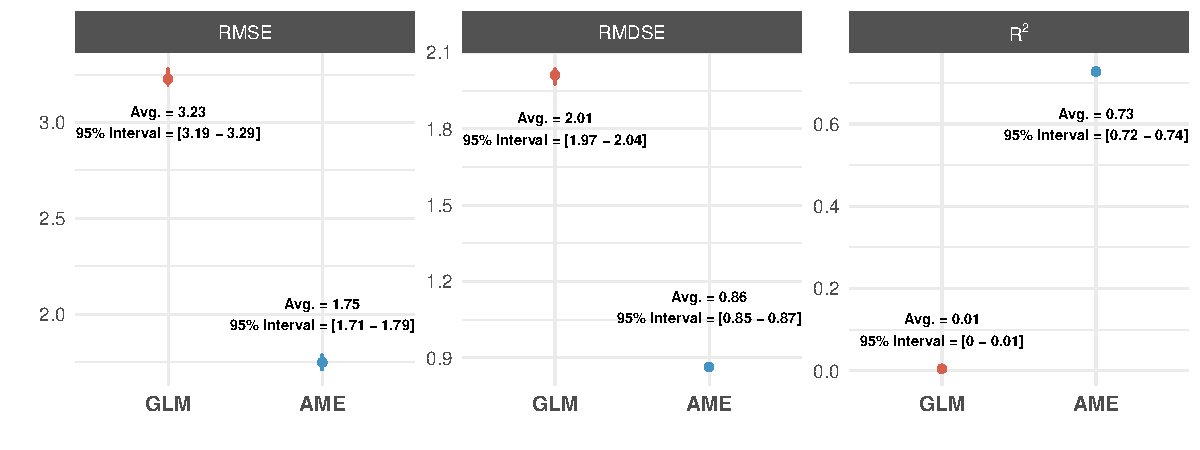
\includegraphics[scale=.5]{roseout}\\
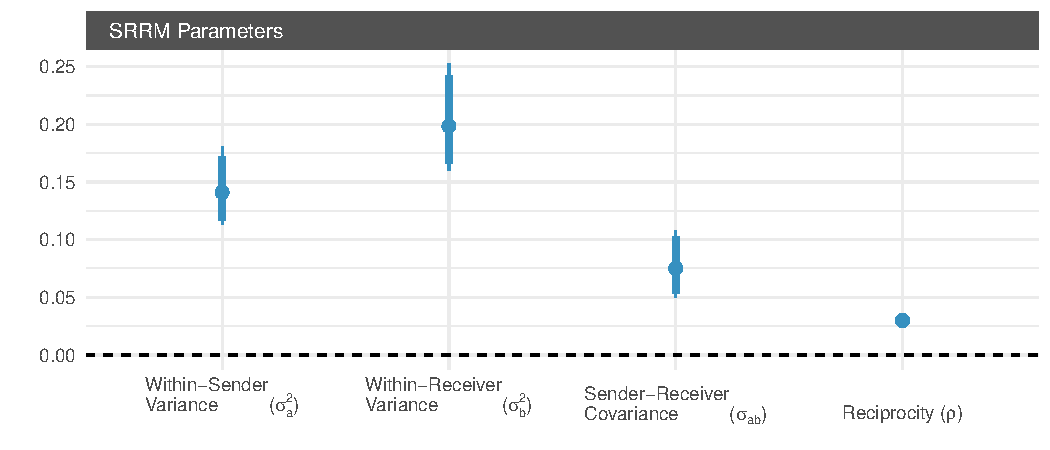
\includegraphics[scale=.4]{rose_srmvc}
\caption{Rose Performance Statistics}
\end{figure}
}

\frame{
  \frametitle{Weeks Performance Comparisons }
  \framesubtitle{ }
\vspace{-5mm}
\begin{figure}
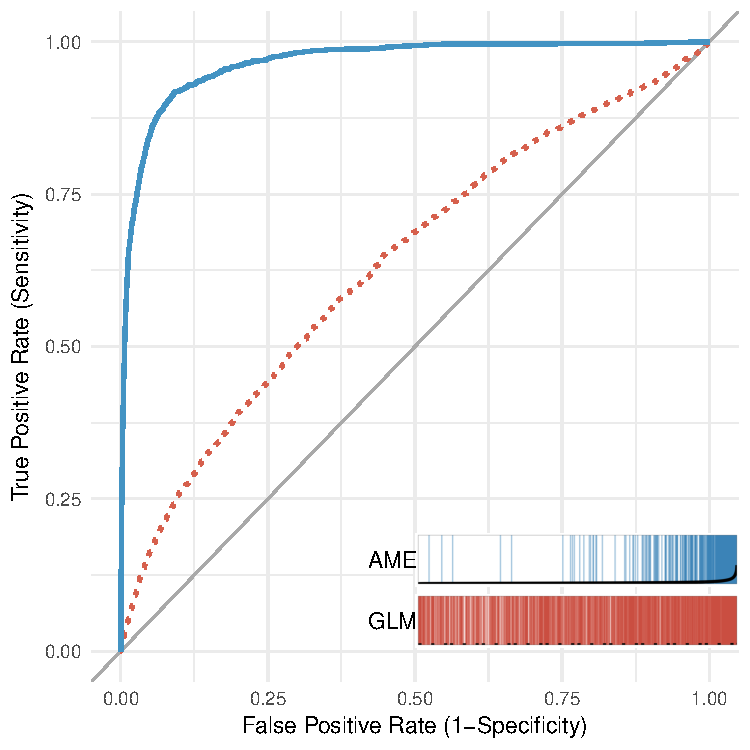
\includegraphics[height=5cm]{weeksroc}
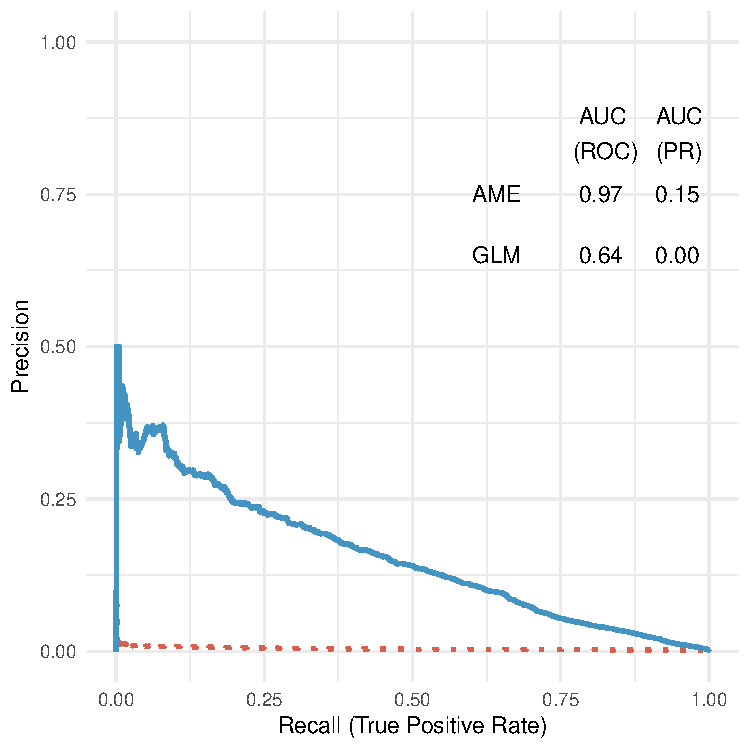
\includegraphics[height=5cm]{weekspr}
\caption{Weeks Performance; no single MID predicted}
\end{figure}
}

\frame{
  \frametitle{Gibler Performance Comparisons }
  \framesubtitle{ }
\vspace{-5mm}
\begin{figure}
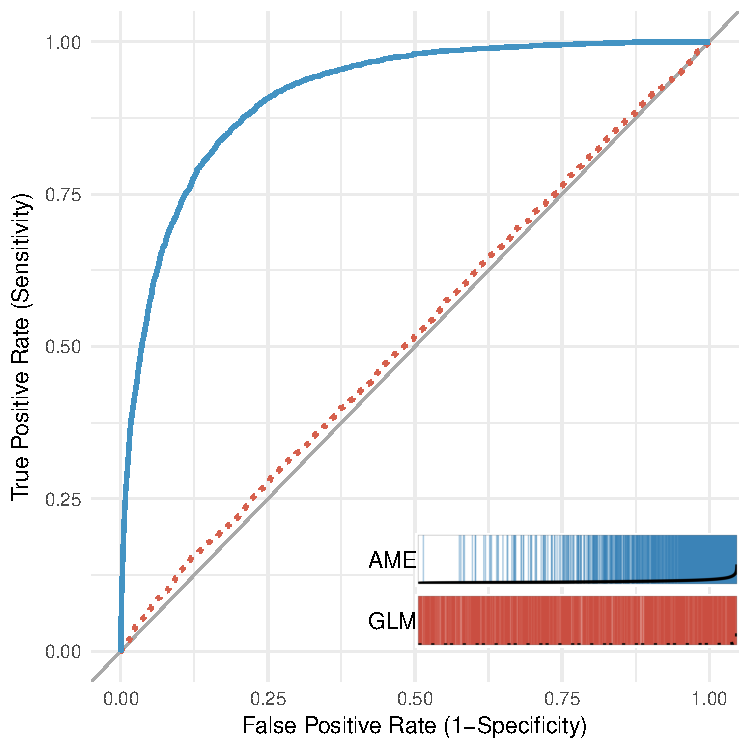
\includegraphics[height=5cm]{giblerroc}
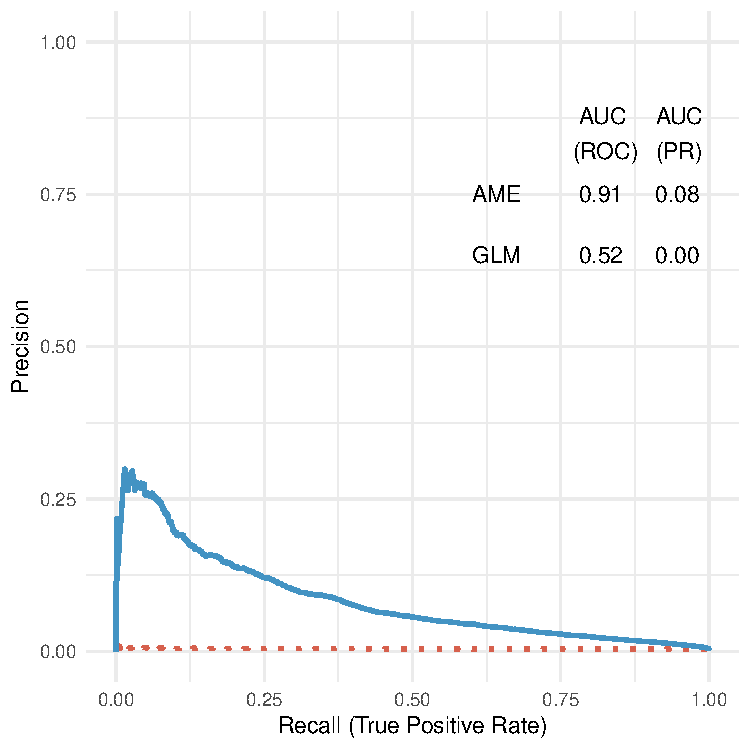
\includegraphics[height=5cm]{giblerpr}
\caption{Gibler Performance; no single MID predicted}
\end{figure}
}

%%%%%%%%%%%%%%%%%%%%%%%
\section{Lessons Learned}
\frame{
   \frametitle{Some Lessons Learned}
  \framesubtitle{ } 
\begin{itemize}
\item Findings that do not take interdependencies into account lose their statistical significance when network effects are estimated via AME. In GLM approaches to the analysis of dyadic data, coefficents are biased, imprecisely measured, and have poorly calibrated standard errors.  This means that significance testing (for better or worse) is compromised when network effects are ignored.
\item New insights emerge from the additional information derived from AME. In particular, there is actual information about the dependencies so that clusters can be identified,   the extent of reciprocity at the dyad level, and among dyads.  
\item The actual results---not the estimated coefficients and their covariances---which are generated by the models differ greatly in expectations.   
\item The AME approach dominates the GLM approaches in terms of performance. Not only it is better at correctly identifying cases in which the dependent variable takes a value of $0$, but it also dominates at correctly identifying occurrences of $1$.     

\end{itemize}
}

\begin{frame}{Frame}
  \frametitle{Networks Really Matter}
  \framesubtitle{We miss a lot when we ignore them.}
  \begin{columns}
    \column{0.5\textwidth}
    \centering
      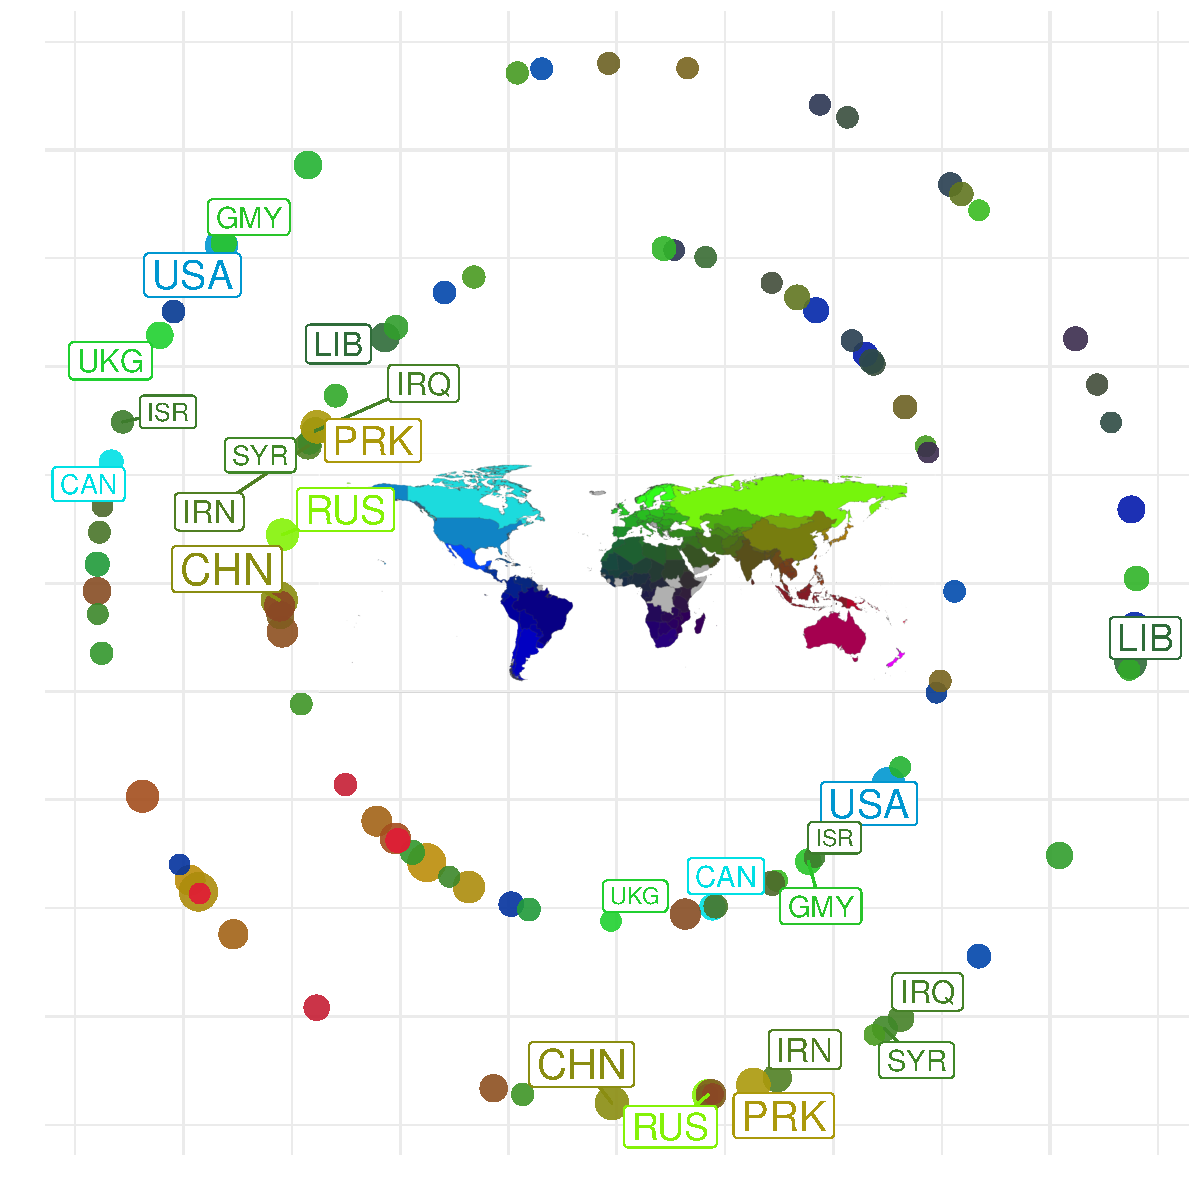
\includegraphics[width=\linewidth]{weeks_circPlot.pdf}
      \column{0.5\textwidth}
      \setlength\arraycolsep{3pt}
      \begin{itemize}
        \item clustering
        \item different patterns for senders and receivers
        \item similar nodal, and dyadic patterns 
        \item gauge reciprocity (and orthogonality)
      \end{itemize}
 \end{columns}
\end{frame}

\frame{\frametitle{Thanks!}
\framesubtitle{There's more, but I'll stop here for your questions and comments.}

More work; copies available upon request:

\begin{itemize}
\item Shahryar Minhas, Peter D. Hoff, and Michael D. Ward. 2017. \textit{Additive and Multiplicative Latent Factor Models for Network Influence}. 
\item Shahryar Minhas, Peter D. Hoff, and Michael D. Ward. 2017. \textit{Influence Networks in International Relations}. 
\item Shahryar Minhas, Cassy L. Dorff, Margaret Foster, Max Gallop, Howard Liu, Juan Tellez, and Michael D. Ward. 2017. \textit{Taking Dyads Seriously}.
\end{itemize}

Thank you!

}
\section{Appendix: Code Example}

\frame{
  \frametitle{Example $\mathcal{R}$ code}
Using the AMEN function requires formatting data into a particular structure. The primary distinction in data formatting is whether the outcome of interest represents a directed or undirected network. Use this link \url{GitHub.com/s7minhas/amen}

If undirected, the AMEN function has three main inputs:

\begin{itemize} 
    \item Y: a $T$ length \textbf{list} of $n\times n$ adjacency matrices, where $T$ = number of years in the dataset and $n$ = number of nodes in the network.
    \item Xdyad: a $T$ length \textbf{list} of $n\times n\times p$ arrays, where $p$ = number of dyadic covariates in dataset. 
    \item Xrow: a $T$ length \textbf{list} of $n\times p$ matrices, where $p$ = number of monadic (nodal) covariates in dataset. 
\end{itemize}

If directed, AMEN further requires: 

\begin{itemize} 
    \item Xrow: a $T$ length list of $n\times p$ matrices, where $p$ = number of sender (nodal) covariates in dataset. 
    \item Xcol: a $T$ length list of $n\times p$ matrices, where $p$ = number of receiver (nodal) covariates in dataset. 
\end{itemize}

}

\frame{
  \frametitle{AMEN Example}
  \framesubtitle{specification}
Beyond the data inputs, the AMEN function requires additional specification: 

\begin{itemize}
    \item model: how to model the outcome variable, e.g., `logit'
    \item symmetric: whether the input network is symmetric
    \item intercept: whether to estimate an intercept
    \item nscan: number of iterations of the Markov chain
    \item burn: burn-in period
    \item odens: thinning interval
    \item R: dimension of the multiplicative effect (referred to as $K$ in the paper)
    \item gof: whether to calculate goodness-of-fit statistics
\end{itemize}

}

\frame{
  \frametitle{Actual Code}
\# running in parallel varying k\\
imps = 10000 ; brn = 25000 ; ods = 10 ; latDims = 0:3\\
\# Run amen in parallel
library(doParallel) ; library(foreach) ; cl=makeCluster(4) \\ registerDoParallel(cl)\\
foreach(ii=1:length(latDims), .packages=c("amen")) \%dopar\% {\\
  \# load previous model run\\
  load(prevModelFiles[ii])\\
  \# extract start vals\\
  startVals0 = ameFit\$'startVals'\\
  \# dump rest\\ 
  rm(ameFit)\\
   ameFit = ame\_repL(\\
    Y=yList,Xdyad=xDyadList,Xrow=NULL,Xcol=NULL, \\
    model="bin",symmetric=FALSE,intercept=TRUE,R=latDims[ii], \\
    nscan=imps, seed=1, burn=brn, odens=ods, \\
    plot=FALSE, print=FALSE, gof=TRUE, startVals=startVals0,\\
    periodicSave=TRUE ) \\    
  save(ameFit, file=paste0('model\_k', latDims[ii],'\_v2.rda') )\\
}
stopCluster(cl)
}
%%%%%%%%%%%%%%%%%%%%%%%%%%%%%%%%%%%%%%%%%%%%%%%%%%%%%%%%%%%%
%\section{Backup Slides}
\frame{\frametitle{backup slides}
Go ahead, ask me about ERGM. }

\frame{
  \frametitle{There is a problem with ERGM.}
  \framesubtitle{It is a bug, not a feature.}
\vspace{-5mm}
It is a bug, not a feature. If you don't believe us, believe these scholars:
\begin{enumerate}
\item Schweinberger, M. (2011). Instability, Sensitivity, and Degeneracy of Discrete Exponential Families. \textbf{Journal of the American Statistical Association}, 106(496):1361–1370.
\item Schweinberger, M. and Handcock, M. S. (2015). Local Dependence in Random Graph Models: Characterization, Properties and Statistical Inference. \textbf{Journal of the Royal Statistical Society: Series B (Statistical Methodology)}, 77(3):647–676.
\item Chatterjee, S. and Diaconis, P. (2013). Estimating and Understanding Exponential Random Graph Models. \textbf{The Annals of Statistics}, 41(5):2428–2461.
\item Rastelli, R., Friel, N., and Raftery, A. E. (2016). Properties of Latent Variable Network Models. \textbf{Network Science}, 4(4):1–26.
\end{enumerate}
}
%%%%%%%%%%%%%%%%%%%%%%%%%%%%%%%%%%%%%%%%%%%%%%%%%%%%%%%%%%%%

%%%%%%%%%%%%%%%%%%%%%%%%%%%%%%%%%%%%%%%%%%%%%%%%%%%%%%%%%%%%
\frame{
  \frametitle{What Is Really Wrong? }
\vspace{-5mm}

You may assume this is your likelihood surface.  Courtesy of Chatterjee and Diaconis, who concluded that sufficient statistics are not sufficient to solve this problem.  Estimation of ERGMs contains this flaw, with pseudolikelihood, maximum likelihood, or MCMC. 
\includegraphics[width=1\textwidth]{disconuity.png}
}
%%%%%%%%%%%%%%%%%%%%%%%%%%%%%%%%%%%%%%%%%%%%%%%%%%%%%%%%%%%%

%%%%%%%%%%%%%%%%%%%%%%%%%%%%%%%%%%%%%%%%%%%%%%%%%%%%%%%%%%%%
\frame{
  \frametitle{What Does This Mean? }
\vspace{-5mm}
\begin{enumerate}
\item Probabilistic ERGM models place almost all of the probability on networks that
are either nearly empty (degenerate) with no linkages or nearly saturated with
all nodes being interconnected. 
\item The likelihood surface contains steep or discontinuous gradients that render it impossible to solve numerically (or analytically). Even (especially) for very small networks this is problematic.
\item Find a different way to estimate network data.  
\end{enumerate}
}
%%%%%%%%%%%%%%%%%%%%%%%%%%%%%%%%%%%%%%%%%%%%%%%%%%%%%%%%%%%%

%%%%%%%%%%%%%%%%%%%%%%%%%%%%%%%%%%%%%%%%%%%%%%%%%%%%%%%%%%%%
\frame{
  \frametitle{Extant Political Science Examples}
\vspace{-5mm}
Extant Political Science Examples Using Latent Distance Models Are Wrong.
\begin{enumerate}
\item There is a problem with the MCMC estimator in \texttt{latentnet}. Don't use it until it is fixed.
\item Latent distance models are hard to correctly interpret, in prominent evaluations in the literature it is done incorrectly.  This is explained in their introduction a decade ago.
\item The advice in Cranmer et al is wrong. Latent network models are not biased and when correctly implemented out-perform ERGM models.
\end{enumerate}
}
%%%%%%%%%%%%%%%%%%%%%%%%%%%%%%%%%%%%%%%%%%%%%%%%%%%%%%%%%%%%
\frame{
\frametitle{Compared to ERGM?}
  \framesubtitle{Swiss Climate Change Application}

Cross-sectional network measuring whether an actor indicated that they collaborated with another during the policy design of the Swiss CO$_{2}$ act (Ingold 2008)

\begin{figure}[ht]
  \centering
  \begin{tabular}{cc}
  \includegraphics[width=.47\textwidth]{dvNet_outDegree} & 
  \includegraphics[width=.44\textwidth]{dvNet_inDegree}
  \end{tabular}
\end{figure}

}
%%%%%%%%%%%%%%%%%%%%%%%%%%%%%%%%%%%%%%%%%%%%%%%%%%%%%%%%%%%%

%%%%%%%%%%%%%%%%%%%%%%%%%%%%%%%%%%%%%%%%%%%%%%%%%%%%%%%%%%%%
\frame{
  \frametitle{Parameter Estimates for Swiss Example}

% latex table generated in R 3.3.1 by xtable 1.8-2 package
% Sun Aug 21 03:32:43 2016
\vspace{-15mm}
\begin{table}[ht]
\centering
\begingroup\scriptsize
\begin{tabular}{lcccccc}
   & Expected & \multirow{2}{*}{Logit} & \multirow{2}{*}{MRQAP} & \multirow{2}{*}{LSM} & \multirow{2}{*}{ERGM} & \multirow{2}{*}{AME} \\ 
   & Effect & & & & & \\
  \hline
  \textbf{Conflicting policy preferences} &  &  &  &  &  &  \\ 
  $\;\;\;\;$ Business vs. NGO & \color{red}{$-$} & -0.86 & \color{red}{-0.87$^{\ast}$} & \color{red}{-1.37$^{\ast}$} & \color{red}{-1.11$^{\ast}$} & \color{red}{-1.37$^{\ast}$} \\ 
  $\;\;\;\;$ Opposition/alliance & \color{blue}{$+$} &  \color{blue}{1.21$^{\ast}$} & \color{blue}{1.14$^{\ast}$} & 0.00 & \color{blue}{1.22$^{\ast}$} & \color{blue}{1.08$^{\ast}$} \\ 
  $\;\;\;\;$ Preference dissimilarity & \color{red}{$-$} & -0.07 & -0.60 & \color{red}{-1.76$^{\ast}$} & -0.44 & \color{red}{-0.79$^{\ast}$} \\ 
  \textbf{Transaction costs} &  &  &  &  &  &  \\ 
  $\;\;\;\;$ Joint forum participation & \color{blue}{$+$} & \color{blue}{0.88$^{\ast}$} & \color{blue}{0.75$^{\ast}$} & \color{blue}{1.51$^{\ast}$} & \color{blue}{0.90$^{\ast}$} & \color{blue}{0.92$^{\ast}$} \\ 
  \textbf{Influence} & &  &  &  &  &  \\ 
  $\;\;\;\;$ Influence attribution & \color{blue}{$+$} & \color{blue}{1.20$^{\ast}$} & \color{blue}{1.29$^{\ast}$} & 0.08 & \color{blue}{1.00$^{\ast}$} & \color{blue}{1.09$^{\ast}$} \\ 
  $\;\;\;\;$ Alter's influence indegree & \color{blue}{$+$} & \color{blue}{0.10$^{\ast}$} & \color{blue}{0.11$^{\ast}$} & 0.01 & \color{blue}{0.21$^{\ast}$} & \color{blue}{0.11$^{\ast}$} \\ 
  $\;\;\;\;$ Influence absolute diff. & \color{red}{$-$} & \color{red}{-0.03$^{\ast}$} & \color{red}{-0.06$^{\ast}$} & 0.04 & \color{red}{-0.05$^{\ast}$} & \color{red}{-0.07$^{\ast}$} \\ 
  $\;\;\;\;$ Alter = Government actor & \color{blue}{$+$} & \color{blue}{0.63$^{\ast}$} & 0.68 & -0.46 & \color{blue}{1.04$^{\ast}$} & 0.55 \\ 
  \textbf{Functional requirements} &  &  &  &  &  & \\ 
  $\;\;\;\;$ Ego = Environmental NGO & \color{blue}{$+$} & \color{blue}{0.88$^{\ast}$} & 0.99 & -0.60 & \color{blue}{0.79$^{\ast}$} & 0.67 \\ 
  $\;\;\;\;$ Same actor type & \color{blue}{$+$} & \color{blue}{0.74$^{\ast}$} & \color{blue}{1.12$^{\ast}$} & \color{blue}{1.17$^{\ast}$} & \color{blue}{0.99$^{\ast}$} & \color{blue}{1.04$^{\ast}$} \\ 
   \hline
\end{tabular}
\endgroup
\end{table}

}
%%%%%%%%%%%%%%%%%%%%%%%%%%%%%%%%%%%%%%%%%%%%%%%%%%%%%%%%%%%%

%%%%%%%%%%%%%%%%%%%%%%%%%%%%%%%%%%%%%%%%%%%%%%%%%%%%%%%%%%%%
\frame{
  \frametitle{Latent Factor Visualization for Swiss Example}

  \centering
  \vspace{-10mm}
  \includegraphics[width=.7\textwidth]{ameFitSR_2_UV}

}
%%%%%%%%%%%%%%%%%%%%%%%%%%%%%%%%%%%%%%%%%%%%%%%%%%%%%%%%%%%%

%%%%%%%%%%%%%%%%%%%%%%%%%%%%%%%%%%%%%%%%%%%%%%%%%%%%%%%%%%%%
\frame{
  \frametitle{Out-of-Sample Performance Assessment: Strategy}

\begin{itemize}
  \item  Randomly divide the $n \times (n-1)$ data points into $S$ sets of roughly equal size, letting $s_{ij}$ be the set to which pair $\{ij\}$ is assigned.
  \item  For each $s \in \{1, \ldots, S\}$:
  \begin{itemize}
    \item  Obtain estimates of the model parameters conditional on $\{y_{ij} : s_{ij} \neq s\}$, the data on pairs not in set $s$.
    \item  For pairs $\{kl\}$ in set $s$, let $\hat y_{kl} = E[y_{kl} | \{y_{ij} : s_{ij} \neq s\}]$, the predicted value of $y_{kl}$ obtained using data not in set $s$.
  \end{itemize}
\end{itemize}

This procedure generates a sociomatrix of out-of-sample predictions of the observed data

}
%%%%%%%%%%%%%%%%%%%%%%%%%%%%%%%%%%%%%%%%%%%%%%%%%%%%%%%%%%%%

%%%%%%%%%%%%%%%%%%%%%%%%%%%%%%%%%%%%%%%%%%%%%%%%%%%%%%%%%%%%
\frame{
  \frametitle{Performance Comparison for Swiss Example}

\begin{tabular}{cc}
\includegraphics[width=.5\textwidth]{roc_outSample} & 
\includegraphics[width=.5\textwidth]{rocPr_outSample} 
\end{tabular}

}
%%%%%%%%%%%%%%%%%%%%%%%%%%%%%%%%%%%%%%%%%%%%%%%%%%%%%%%%%%%%

%%%%%%%%%%%%%%%%%%%%%%%%%%%%%%%%%%%%%%%%%%%%%%%%%%%%%%%%%%%%
\frame{
  \frametitle{Network Dependencies: Swiss Example}
  \centering
  \includegraphics[width=1\textwidth]{netPerfCoef}

}

%%%%%%%%%%%%%%%%%%%%%%%%%%%%%%%%%%%%%%%%%%%%%%%%%%%%%%%%%%%%
\frame{
  \frametitle{Much current advice is wrong.}
  \textbf{Unfortunately some misleading and incorrect advice is in the current literature. Maybe it will be corrected.}

\begin{enumerate}
\item Cranmer, Leifeld, McClurg, Rolfe (2017 AJPS) stated that latent space models are only preferable if there are few isolates, enough observations, and the interdependence is theoretically uninteresting. 

\item All of this is wrong. Not only do they incorrectly assume all latent models to be based on Euclidean distance but their statistical comparisons are based on a program that contains known errors. Moreover, using BIC to choose among different network models is itself questionable.

\item It is not true that ``ERGM offers the most preferable combination of model fit and number of parameters,'' despite their assertions.
\end{enumerate}
}
%%%%%%%%%%%%%%%%%%%%%%%%%%%%%%%%%%%%%%%%%%%%%%%%%%%%%%%%%%%%



%%%%%%%%%%%%%%%%%%%%%%%%%%%%%%%%%%%%%%%%%%%%%%%%%%%%%%%%%%%%
\frame{
  \frametitle{Simulation Comparison}

\includegraphics[width=1\textwidth]{ameVergmSim.png}

}
%%%%%%%%%%%%%%%%%%%%%%%%%%%%%%%%%%%%%%%%%%%%%%%%%%%%%%%%%%%%

%%%%%%%%%%%%%%%%%%%%%%%%%%%%%%%%%%%%%%%%%%%%%%%%%%%%%%%%%%%%
\frame{
  \frametitle{AMEN v LSM Performance}

  \begin{tabular}{cc}
  \includegraphics[width=.5\textwidth]{roc_latSpace_outSample} & 
  \includegraphics[width=.5\textwidth]{rocPr_latSpace_outSample}
  \end{tabular}

}
%%%%%%%%%%%%%%%%%%%%%%%%%%%%%%%%%%%%%%%%%%%%%%%%%%%%%%%%%%%%

%%%%%%%%%%%%%%%%%%%%%%%%%%%%%%%%%%%%%%%%%%%%%%%%%%%%%%%%%%%%
\frame{
  \frametitle{AMEN versus LSM Net Dependence}

  \includegraphics[width=1\textwidth]{netPerfCoef_latSpace}
}
%%%%%%%%%%%%%%%%%%%%%%%%%%%%%%%%%%%%%%%%%%%%%%%%%%%%%%%%%%%%

%%%%%%%%%%%%%%%%%%%%%%%%%%%%%%%%%%%%%%%%%%%%%%%%%%%%%%%%%%%%
\frame{
  \frametitle{AMEN varying $K$ Performance}

  \begin{tabular}{cc}
  \includegraphics[width=.5\textwidth]{roc_ameSR_outSample} & 
  \includegraphics[width=.5\textwidth]{rocPr_ameSR_outSample}
  \end{tabular}

}
%%%%%%%%%%%%%%%%%%%%%%%%%%%%%%%%%%%%%%%%%%%%%%%%%%%%%%%%%%%%

%%%%%%%%%%%%%%%%%%%%%%%%%%%%%%%%%%%%%%%%%%%%%%%%%%%%%%%%%%%%
\frame{
  \frametitle{AMEN varying $K$ Net Dependence}

  \includegraphics[width=1\textwidth]{netPerfCoef_ameSR}
}
%%%%%%%%%%%%%%%%%%%%%%%%%%%%%%%%%%%%%%%%%%%%%%%%%%%%%%%%%%%%

\end{document}
